\chapter{Planteamiento del problema}
El sedentarismo es una de las principales causas de la obesidad y sobrepeso en Guatemala, as\'i mismo constituyen un factor determinante para el desarrollo de enfermedades cr\'onicas no transmisibles, concretamente la diabetes, tal como se muestra en el estudio m\'edico sobre el riesgo de desarrollar diabetes tipo 2 en Guatemala  \cite{castro2017risk}, menciona que el 47\% de los guatemaltecos con diabetes tienen problemas de obesidad y el 31\%  sufren de problemas de sobrepeso, por lo cual refleja la inactividad f\'isica en una gran parte de la poblaci\'on guatemalteca.
\medbreak
Por otra parte, se ha reducido el nivel de actividad f\'isica en las personas guatemaltecas, de acuerdo con la encuesta de diabetes, hipertensi\'on y factores de riesgo de enfermedades cr\'onicas \cite{orellana2006organizacion}, el 27.68\% de los guatemaltecos presentan sedentarismo, debido que no realizan actividades f\'isicas o lo hacen por menos de 30 minutos al d\'ia.
\medbreak
Igualmente, se realiz\'o un estudio a 392 ni\~nos y adolescentes en escuelas rulares y urbanas de Guatemala \cite{muros2016doble}, en donde indica que alrededor del 62\% de los ni\~nos del  \'area urbana presentan problemas de sobrepeso y un 13.8\% de obesidad, de modo que los autores concluyeron que el sobrepeso y la obesidad coexisten en los ni\~nos y adolescentes guatemaltecos.
\medbreak
En resumen, el presente proyecto busca detectar que un usuario se mueva a partir de repeticiones de un movimiento, de tal modo de responder la siguiente pregunta:
\medbreak
\begin{center}
\textbf{?`Ser\'a posible detectar el movimiento de una persona durante una actividad f\'isica?}
\end{center}
\section{OBJETIVOS}
\subsection{OBJETIVO GENERAL}
Realizar una m\'quina de aprendizaje demostrativa que registre el seguimiento de esqueleto (Skeletan traking) a trav\'es de una c\'amara con sensor de profundidad, seleccionando el mejor modelo matem\'atico, con la finalidad de detectar los pasos que se requiere para realizar un movimiento funcional.
\subsection{OBJETIVOS ESPEC�FICOS}
\begin{enumerate}[1.]
    \item Identificar la altura correcta de la c\'amara y la distancia entre el usuario y el dispositivo para detectar el seguimiento del esqueleto humano.
    \item Analizar los kits de desarrollo de software (SDK) que permite grabar v\'ideos, tomar fotograf\'ias y capturar el seguimiento de esqueleto a trav\'es de una c\'amara con sensor de profundidad.
    \item Crear una interfaz gr\'afica que capture los datos de los pasos que deben seguir para realizar un movimiento funcional.
    \item Recolectar y validar los datos de entrenamiento de los movimientos funcionales.
    \item Identificar y comparar distintos modelos matem\'ticos a partir de los datos recolectado.
    \item Seleccionar el mejor modelo matem\'atico a partir de su rendimiento algor\'itmico y menor porcentaje de falla.
    \item Validar el modelo matem\'atico. 
    \item Crear una interfaz gr\'afica que detecte los pasos que se deben seguir para realizar un movimiento funcional.
\end{enumerate}
\section{HIP�TESIS}
\section{Variables} \label{vr}
\subsection{Primer Objetivo} \label{vr:1o}
Por movimiento se debe enumerar las articulaciones que ayudan a un usuario a moverse, de igual manera, por cada movimiento se debe enumerar los pasos que se debe seguir para ejecutar la acci\'on -i.e. Repetici\'on del movimiento-.
\subsubsection{Variables dependientes} \label{vr:1o:dep}
\begin{enumerate}
	\item[A.] \textbf{Articulaciones del movimiento:}  Vector de enteros la cual se almacena el valor del enumerador, JointType, del SDK de  \citeA{microsoftJointKinect}.
	\item[B.] \textbf{N\'umeros de pasos}: Valor positivo, mayor a 1.
\end{enumerate}
	\begin{figure}[H]
	\caption{Variables dependientes del primer objetivo}
	\label{fig:vardep1}
	\centering
	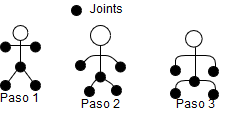
\includegraphics[width=300px,height=100px]{graphics/var-1obj.png} \\
	\textbf{Fuente:}Elaboraci\'on propia 
\end{figure}
\medbreak
\begin{table}[H]
\begin{center}
\caption{Definiciones de variables dependientes del primer objetivo}
\label{tab:def1o}
\begin{tabular}{|l|l|l|}
\hline
Enumeraci\'on & Definici\'on Operacional & Definici\'on conceptual \\
\hline
\ref{vr:1o:dep}.A & \begin{tabular}[c]{@{}l@{}}Son aquellas articulaciones\\ que interviene para realizar\\ el movimiento -i.e. Arcos\\ de movibilidad-.\end{tabular} & \begin{tabular}[c]{@{}l@{}}Conjunto de \'indices enteros \\ que representa las articulaciones\\ (ver figura \ref{fig:jointsKinect}) y arcos de\\ movibilidad (ver figuras \ref{fig:ArcosdeMovilidad} y \ref{fig:ArcosdeMovilidad2})\\ del seguimiento del esqueleto \end{tabular}  \\
\hline
\ref{vr:1o:dep}.B & \begin{tabular}[c]{@{}l@{}}Cantidad de pasos de an\'alisis\\ que tiene el movimiento\end{tabular} & \begin{tabular}[c]{@{}l@{}}De acuerdo a las variables del \\  movimiento (ver secci\'on \ref{mt:mf:var}), \\ los pasos define la coordinaci\'on \\ y balance del movimiento\end{tabular}\\
\hline
\end{tabular}
\end{center}
\textbf{Fuente:} Elaborado por el autor de tesis
\end{table}
\subsection{Tercer Objetivo} \label{vr:3o}
Por cada movimiento es necesario indicar la articulaci\'on de an\'alisis -i.e. Punto central de estudio-,  la cual a partir de ella se calcula la distancia de profundidad m\'inima y m\'axima, con la finalidad de que el seguimiento de esqueleto tenga un menor posible, sin embargo esta funcionalidad depende de la altura de usuario y el Kinect. 
\subsubsection{Variables dependientes} \label{vr:3o:dep}
\begin{enumerate}
	\item[A.] \textbf{Articulaci\'on de an\'alisis}: Valor entero que pertenece al  enumerador, JointType, del SDK de \citeA{microsoftJointKinect}. 
	\item[B.] \textbf{Altura del usuario}: Valor decimal positivo -i.e. Medida en metros- que se determina a partir de los componentes de altura de las articulaciones de la cabeza y p\'ies del usuario.	
	\begin{formula}[h]
	\centering
	\caption{Altura del usuario}
	\label{frm:alturaUser}
	\begin{equation}
y_{usuario}=y_{cabeza}-\frac{y_{pieDerecho}+y_{pieIzquierdo}}{2}
	\end{equation}
			\textbf{Fuente:} Planteado por el autor de tesis
\end{formula}  
	\item[C.] \textbf{Altura del kinect respecto al suelo}: Valor decimal positivo -i.e. Medida en metros- que permanece constante por movimiento. 
\end{enumerate}
\medbreak
\begin{figure}[H]
	\caption{Variables dependientes del tercer objetivo}
	\label{fig:vardep3}
	\centering
	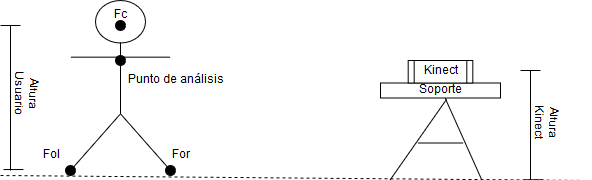
\includegraphics[width=300px,height=100px]{graphics/var-3obj.png} \\
	\textbf{Fuente:}Elaboraci\'on propia 
\end{figure}
\medbreak
\begin{table}[H]
\begin{center}
\caption{Definiciones de variables dependientes del Tercer objetivo}
\label{tab:def3o}
\begin{tabular}{|l|l|l|}
\hline
Enumeraci\'on & Definici\'on Operacional & Definici\'on conceptual \\
\hline
\ref{vr:3o:dep}.A & \begin{tabular}[c]{@{}l@{}}Articulaci\'on que ayuda\\ a determinar las distancias\\ m\'aximas y m\'inimas\\ de profundidad, adem\'as de\\ calcular el recorrido del atleta \\ durante la repetici\'on del movimiento\end{tabular} & \begin{tabular}[c]{@{}l@{}}Articulaci\'on del seguimiento de \\ de esqueleto (ver figura \ref{fig:jointsKinect}), que\\ permite realizar el an\'alisis del movimiento,\\ tal como se muestra en los trabajos \\ relacionados (Ver secci\'on \ref{tr}) \end{tabular}  \\
\hline
\ref{vr:3o:dep}.B & \begin{tabular}[c]{@{}l@{}}Variable de referencia para \\ ubicar al usuario en la profundidad \\ adecuada del seguimiento \\ del esqueleto\end{tabular} & \begin{tabular}[c]{@{}l@{}}La altura es una variable que puede \\ afectar los movimientos cinem\'aticos \\ (ver secci\'on \ref{mt:cam:kin}.\ref{mt:cam:kin:vgb}), \\ dado que afecta las dimenciones \\ del seguimiento de esqueleto\end{tabular}\\
\hline
\ref{vr:3o:dep}.C & \begin{tabular}[c]{@{}l@{}}Variable que permanece constante\\ por movimiento, adem\'as de ser \\ el punto central de  \\ captura de datos del Kinect\end{tabular} & \begin{tabular}[c]{@{}l@{}}La transmici\'on de datos del Kinect \\ (ver figura \ref{fig:interaccionKinect}) tendr\'a un menor error, \\  si se posiciona a la altura \\ en donde el sensor tenga un \\  mayor campo de visi\'on (ver figura \ref{fig:RGBESP} ) \end{tabular}\\
\hline
\end{tabular}
\end{center}
\textbf{Fuente:} Elaborado por el autor de tesis
\end{table}
\subsubsection{Variables independientes} \label{vr:3o:indep}
\begin{enumerate}
	\item[A.] \textbf{Distancia m\'inima de profundidad del movimiento}: Valor decimal positivo -i.e. Medida en metros- que determina la distancia m\'inima adecuada para ejecutar el seguimiento de esqueleto.
	\item[B.] \textbf{Distancia m\'axima de profundidad del movimiento}: Valor decimal positivo -i.e. Medida en metros- que determina la distancia m\'axima adecuada para ejecutar el seguimiento de esqueleto.
\end{enumerate}
\medbreak
\begin{figure}[H]
	\caption{Variables independientes del tercer objetivo}
	\label{fig:varindep3}
	\centering
	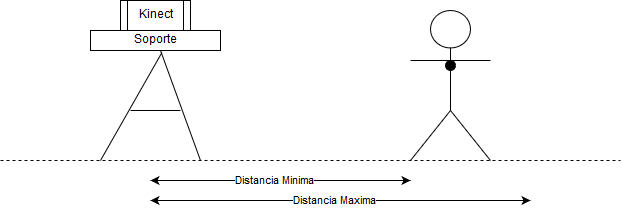
\includegraphics[width=300px,height=100px]{graphics/var-3obj-ind.png} \\
	\textbf{Fuente:}Elaboraci\'on propia 
\end{figure}
\medbreak
\begin{table}[H]
\begin{center}
\caption{Definiciones de variables independientes del Tercer objetivo}
\label{tab:def3o2}
\begin{tabular}{|l|l|l|}
\hline
Enumeraci\'on & Definici\'on Operacional & Definici\'on conceptual \\
\hline
\ref{vr:3o:indep}.A & \begin{tabular}[c]{@{}l@{}}Distancia m\'inima la\\ cual detecta todo el\\ esqueleto del usuario\\ -i.e. desde la cabeza \\ hasta los p\'ies-.\end{tabular} & \multirow{2}{*}{\begin{tabular}[c]{@{}l@{}} El seguimiento de esqueleto\\ depende del alcance del sensor \\ de profundidad y el campo \\ de visi\'on (ver figura \ref{fig:RGBESP}). \end{tabular}} \\
\cline{1-2}
\ref{vr:3o:indep}.B & \begin{tabular}[c]{@{}l@{}}Distancia m\'axima la\\ cual deja de detectar\\ todo el esqueleto del \\  usuario. \end{tabular} & \\
\hline
\end{tabular}
\end{center}
\textbf{Fuente:} Elaborado por el autor de tesis
\end{table}
\subsection{Cuarto Objetivo} \label{vr:4o}
Durante un movimiento, una articulaci\'on se desplaza con una direcci\'on - i.e. En todos los sentidos-, durante un per\'iodo de tiempo.
\subsubsection{Variables dependientes} \label{vr:4o:dep}
\begin{enumerate}
	\item[A.] \textbf{Tiempo de captura de datos}: Valor decimal positivo -i.e. Medida en segundos-, la cual mide el tiempo del movimiento de una articulaci\'on.
\end{enumerate}
\medbreak
\begin{figure}[H]
	\caption{Variables dependientes del cuarto objetivo}
	\label{fig:vardep4}
	\centering
	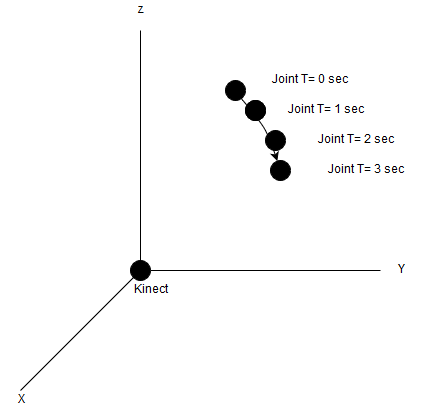
\includegraphics[width=180px,height=100px]{graphics/var-4obj.png} \\
	\textbf{Fuente:}Elaboraci\'on propia 
\end{figure}
\begin{table}[H]
\begin{center}
\caption{Definiciones de variables dependientes del cuarto objetivo}
\label{tab:def4o}
\begin{tabular}{|l|l|l|}
\hline
Enumeraci\'on & Definici\'on Operacional & Definici\'on conceptual \\
\hline
\ref{vr:4o:dep}.A & \begin{tabular}[c]{@{}l@{}}Unidad de tiempo \\  con respecto al \\ movimiento de an\'alisis\end{tabular} & \begin{tabular}[c]{@{}l@{}}De acuerdo a la resoluci\'on de 3D  \\ y del color (ver tabla \ref{tab:RGBD}), \\ el Kinect percibe un total \\ 30 frames por segundos, \\ lo cual puede llegar a  \\  capturar los datos cada \\  0.033 segundos. \end{tabular}  \\
\hline
\end{tabular}
\end{center}
\textbf{Fuente:} Elaborado por el autor de tesis
\end{table}
\subsubsection{Variables independientes} \label{vr:4o:indep}
\begin{enumerate}
	\item[A.] \textbf{Desplazamiento de la articulaci\'on}: Valor decimal positivo -i.e. Medida en metros- que determina la distancia de una articulac\'on y un punto de origen -i.e. Kinect-:
\begin{formula}[h]
	\centering
	\caption{desplazamiento de una articulaci\'on}
	\label{frm:desplazaUser}
	\begin{equation}
|r|=\sqrt{(x_{joint}-x_{o})^{2}+(y_{joint}-y_{o})^{2}+(z_{joint}-z_{o})^{2}}
	\end{equation}
	\textbf{Fuente:} Distancia euclediana \cite[p.~423]{ayres2001calculo}
\end{formula}  
	\item[B.] \textbf{Orientaci\'on de la articulaci\'on}: Vector de valores decimales positivo -i.e. Medida en radianes- que determina el \'angulo del desplazamiento con respecto a sus ejes.
\begin{formula}[h]
	\centering
	\caption{Orientaci\'on de una articulaci\'on}
	\label{frm:orientUser}
	\begin{equation}
Orientacion = [\alpha ,\beta ,\gamma ] = [cos^{-1}(\frac{x_{joint}}{|r|}),cos^{-1}(\frac{y_{joint}}{|r|}),cos^{-1}(\frac{z_{joint}}{|r|})]
	\end{equation}
	\textbf{Fuente:} \'Angulos directores de un vector \cite[p.~424]{ayres2001calculo}
\end{formula}  
\end{enumerate}
\medbreak
\begin{figure}[H]
	\caption{Variables independientes del cuarto objetivo}
	\label{fig:varIdep4}
	\centering
	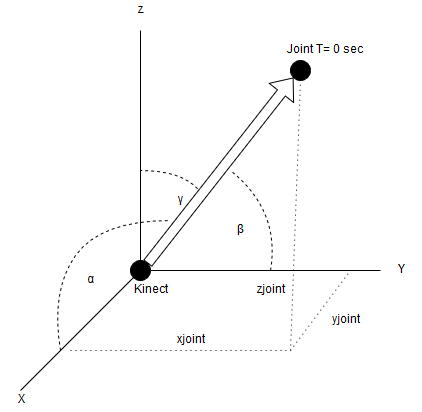
\includegraphics[width=230px,height=150px]{graphics/var-4obj-ind.png} \\
	\textbf{Fuente:}Elaboraci\'on propia 
\end{figure}
\begin{table}[H]
\begin{center}
\caption{Definiciones de variables independientes del cuarto objetivo}
\label{tab:def4oI}
\begin{tabular}{|l|l|l|}
\hline
Enumeraci\'on & Definici\'on Operacional & Definici\'on conceptual \\
\hline
\ref{vr:4o:indep}.A & \begin{tabular}[c]{@{}l@{}}Valor que muestra el desplazamiento \\ de la articulaci\'on de an\'alisis \\ -i.e. Como se esta \\ moviendo el cuerpo-. \end{tabular} & \begin{tabular}[c]{@{}l@{}}De acuerdo a las variables \\ de un movimiento (ver secci\'on \ref{mt:mf:var}) \\ y movimientos cin\'ematicos  \\ (ver secci\'on \ref{mt:cam:kin}.\ref{mt:cam:kin:vgb}),  \\ el desplazamiento permite calcular \\ la velocidad y aceleraci\'on \\ de un movimiento \\ a partir de la posici\'on  \\ de una articulaci\'on \\ (ver figura  \ref{fig:CoordenadaJoint})\\ con respecto al \\ tiempo de movimiento \end{tabular}  \\
\hline
\ref{vr:4o:indep}.B & \begin{tabular}[c]{@{}l@{}}Valor que muestra la direcci\'on   \\ de la articulaci\'on\end{tabular} & \begin{tabular}[c]{@{}l@{}}De acuerdo a las variables \\ de un movimiento (ver secci\'on \ref{mt:mf:var}), \\ la orientaci\'on permite tener mayor \\  precisi\'on y coordinaci\'on al \\  momento de ejecutar un \\  movimiento \end{tabular}  \\
\hline
\end{tabular}
\end{center}
\textbf{Fuente:} Elaborado por el autor de tesis
\end{table}
\subsection{Quinto Objetivo} \label{vr:5o}
Por cada movimiento se le debe asignar una etiqueta a cada paso, esto permite obtener el factor de movimiento -i.e. Pron\'ostico del modelo de reconocimiento de gesturas-.
\subsubsection{Variables dependientes} \label{vr:5o:dep}
\begin{enumerate}
	\item[A.] \textbf{Etiquetas}: Vector de valores decimales entre 0 a 1. Se debe tomar en cuenta que la diferencia entre dos etiquetas seguidas, es igual o cercano al valor de offset -i.e. Valor decimal que representa la distribuci\'on de pasos-.  
\end{enumerate}	
\medbreak
\begin{formula}[h]
	\centering
	\caption{Offset de etiquetas}
	\label{frm:offsetEt}
	\begin{equation}
offset = \frac{1}{pasos-1}
	\end{equation}
	\textbf{Fuente:} Propuesto por el autor de tesis
\end{formula}
\medbreak
\begin{formula}[h]
	\centering
	\caption{Asignaci\'on de etiquetas}
	\label{frm:vecEtiq}
	\begin{equation}
\begin{matrix}
etiquetas=[0, etiqueta(1), ..., etiqueta(paso), ..., 1],\; donde
\\
\\
etiqueta(paso) =
\left\{\begin{matrix}
0 & si\; es\; el\; primer \; paso
\\
etiqueta(paso-1)+offset & si\; es\; un\; paso\; intermedio
\\ 
1 & si\; es\; el\; ultimo\; paso
\end{matrix}\right.
\end{matrix}
	\end{equation}
	\textbf{Fuente:} Propuesto por el autor de tesis
\end{formula}  
\medbreak
\begin{figure}[H]
	\caption{Variables dependientes del quinto objetivo}
	\label{fig:vardep5}
	\centering
	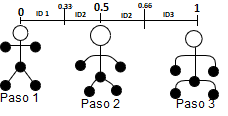
\includegraphics[width=180px,height=100px]{graphics/var-5obj.png} \\
	\textbf{Fuente:}Elaboraci\'on propia 
\end{figure}
\medbreak
\begin{table}[H]
\begin{center}
\caption{Definiciones de variables dependientes del quinto objetivo}
\label{tab:def5oI}
\begin{tabular}{|l|l|l|}
\hline
Enumeraci\'on & Definici\'on Operacional & Definici\'on conceptual \\
\hline
\ref{vr:5o:dep}.A & \begin{tabular}[c]{@{}l@{}}Valor que identifica \\ el paso de un movimiento. \end{tabular} & \begin{tabular}[c]{@{}l@{}}De acuerdo a las variables \\ de un movimiento (ver secci\'on \ref{mt:mf:var}) \\  los coordinaci\'on hace referencia \\ a las etiquetas del movimiento \\ (ver figura \ref{fig:modeloContinuo}). \end{tabular}  \\
\hline
\end{tabular}
\end{center}
\textbf{Fuente:} Elaborado por el autor de tesis
\end{table}
\subsubsection{Variables independientes} \label{vr:5o:indep}
\begin{enumerate}
	\item[A.] \textbf{Factor de movimiento}: valor  decimal entre 0 a 1, la cual representa la probabilidad del seguimiento de un movimiento.
\end{enumerate}	
\medbreak
\begin{figure}[H]
	\caption{Variables independientes del quinto objetivo}
	\label{fig:varIdep5}
	\centering
	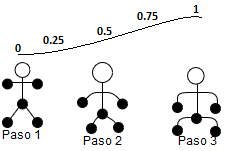
\includegraphics[width=180px,height=100px]{graphics/var-5obj-ind.png} \\
	\textbf{Fuente:}Elaboraci\'on propia 
\end{figure}
\medbreak
\begin{table}[H]
\begin{center}
\caption{Definiciones de variables independientes del quinto objetivo}
\label{tab:def5oI}
\begin{tabular}{|l|l|l|}
\hline
Enumeraci\'on & Definici\'on Operacional & Definici\'on conceptual \\
\hline
\ref{vr:5o:indep}.A & \begin{tabular}[c]{@{}l@{}}Valor que identifica \\ el seguimiento del movimiento \\ en tiempo real \end{tabular} & \begin{tabular}[c]{@{}l@{}}Variable que se calcula  \\ a partir del modelo Random  \\ Forest Regression (ver \\ seccio\'n \ref{mt:cam:kin}.\ref{mt:cam:kin:vgb}) \end{tabular}  \\
\hline
\end{tabular}
\end{center}
\textbf{Fuente:} Elaborado por el autor de tesis
\end{table}
\subsection{S\'eptimo Objetivo} \label{vr:7o}
Una rutina es configurada a partir de un n\'umero de series de tiempo de trabajo y descanso, en donde el usuario realiza las m\'aximas repeticiones posibles del movimiento  durante el tiempo de trabajo, tomando en cuenta que la repetici\'on debe pasar por todos los pasos definidos (ver variable \ref{vr:1o:dep}.B).
\subsubsection{Variables dependientes} \label{vr:7o:dep}
\begin{enumerate}
	\item[A.] \textbf{Tiempo de descanso}: Valor entero positivo -i.e. Medida en segundos-, la cual debe ser menor o igual al tiempo de trabajo.
	\item[B.] \textbf{Tiempo de Trabajo}: Valor entero positivo -i.e. Medida en segundos-.
	\item[C.] \textbf{Cantidad de series}: Valor entero positivo mayor a cero.
\end{enumerate}	
\begin{figure}[H]
	\caption{Variables dependientes del s\'eptimo  objetivo}
	\label{fig:vardep7}
	\centering
	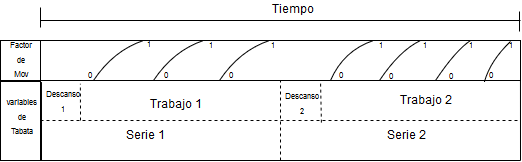
\includegraphics[width=300px,height=100px]{graphics/var-7obj.png} \\
	\textbf{Fuente:}Elaboraci\'on propia 
\end{figure}
\medbreak
\begin{table}[H]
\begin{center}
\caption{Definiciones de variables dependientes del s\'eptimo objetivo}
\label{tab:def7}
\begin{tabular}{|l|l|l|}
\hline
Enumeraci\'on & Definici\'on Operacional & Definici\'on conceptual \\
\hline
\ref{vr:7o:dep}.A & \begin{tabular}[c]{@{}l@{}}Valor que controla el \\ tiempo que debe descansar \\ un usuario durante \\ su rutina -i.e. No \\ se cuenta repeticiones-. \end{tabular} & \multirow{3}{*}{\begin{tabular}[c]{@{}l@{}}Estas variables son \\  definidas a partir de \\ la rutina, Tabata, debido \\ que es un entrenamiento controlado \\  de alta intensidad, \\ cuyo resultado es \\ una mayor metabolizaci\'on \\ del cuerpo  (ver secci\'on \ref{mt:mf:rut}.\ref{mt:mf:rut:hiit})\end{tabular}} \\  
\cline{1-2}
\ref{vr:7o:dep}.B & \begin{tabular}[c]{@{}l@{}}Valor que controla el \\ tiempo que debe trabajar \\ un usuario durante \\ su rutina -i.e. Realizar \\ las m\'aximas repeticiones-. \end{tabular} & \\  
\cline{1-2}
\ref{vr:7o:dep}.C & \begin{tabular}[c]{@{}l@{}}Valor que controla la \\ cantidad de tiempos de \\ trabajos y descanso \\ en una rutina. \end{tabular} &  \\  
\hline
\end{tabular}
\end{center}
\textbf{Fuente:} Elaborado por el autor de tesis
\end{table}
\subsubsection{Variables independientes} \label{vr:7oi:indep}
\begin{enumerate}
	\item[A.] \textbf{Detalle del paso}: Es un vector de valores n\'umericos, en donde contiene el factor de movimiento, n\'umero de paso y la matriz de articulaciones -i.e. Esqueleto-. 
	\item[B.] \textbf{Repetici\'on}:  Es un vector de detalle de todos los pasos definido por el movimiento.
\end{enumerate}	
\begin{formula}[h]
	\centering
	\caption{Matriz de variables independientes del s\'eptimo objetivo}
	\label{frm:vecEtiq}
	\begin{equation}
\begin{matrix}
i & enumerador\: de\: la\: articulacion \\ 
x & distancia\, horizontal \: (pixeles) \\ 
y & distancia\, vertical\: (pixeles) \\ 
joint_{i}& [i,x,y] \\ 
 & \\ 
esqueleto & \begin{bmatrix}
joint_{0} \\ 
... \\ 
joint_{i}\\ 
... \\ 
joint_{24}
\end{bmatrix}  \\ 
 & \\ 
fm & factor \, del \, movimiento \\ 
p  & paso \, del \,movimiento \\ 
step_{p}  & [fm,p,esqueleto, tiempo] \\
 & \\ 
Repeticion & [step_{0}, ...,  step_{col}, ..., step_{last}] \\
serie & [repeticion] \\
series & [serie]
\end{matrix}
	\end{equation}
	\textbf{Fuente:} Propuesto por el autor de tesis
\end{formula}  
\medbreak
\begin{table}[H]
\begin{center}
\caption{Definiciones de variables independientes del s\'eptimo objetivo}
\label{tab:defoi7}
\begin{tabular}{|l|l|l|}
\hline
Enumeraci\'on & Definici\'on Operacional & Definici\'on conceptual \\
\hline
\ref{vr:7oi:indep}.A & \begin{tabular}[c]{@{}l@{}}Variable que almacena informaci\'on \\ del esqueleto humano \\ -i.e. posici\'on de cada \\ articulaci\'on-, con respecto \\  a cada paso del movimiento  \end{tabular} &  \begin{tabular}[c]{@{}l@{}}El seguimiento de esqueleto \\ puede ser dibujado en \\ una imagen 2D (ver figura \ref{fig:skeletanTracking}), \\  la cual proporciona \\ la posici\'on de cada articulaci\'on, \\ con el fin objetivo  de \\ calcular la agilidad \\ del movimiento (ver secci\'on \ref{mt:mf:var})\end{tabular}\\
\hline
\ref{vr:7oi:indep}.B & \begin{tabular}[c]{@{}l@{}}Variable que almacena informaci\'on \\ de todos los pasos \\ en orden cronol\'ogico  \\ -e.g. la informaci\'on del paso 1 \\ es guardada antes del paso 2-. \\ Se debe tomar en cuenta \\ que la repetici\'on ser\'a \\ contable, si tiene todos \' los pasos  \end{tabular} & \begin{tabular}[c]{@{}l@{}}Variable que permite \\ contabilizar la actividad \\ f\'isica de una persona  \\  (ver secci\'on \ref{mt:af:var})\end{tabular}\\  
\hline
\end{tabular}
\end{center}
\textbf{Fuente:} Elaborado por el autor de tesis
\end{table}
\subsection{Octavo Objetivo} \label{vr:8o}
En cada paso del movimiento, los m\'usculos se mueve a partir del arco del  movilidad. 
\subsubsection{Variables independientes} \label{vr:8oi:indep}
\begin{enumerate}
	\item[A.] \textbf{Flexibilidad}: Valor decimal positivo -i.e. Medida en grados-, la cual mide el \'angulo de una articulaci\'on respecto a 2 articulaciones continuas.
\end{enumerate}	
\begin{figure}[H]
	\caption{Variables independiente del octavo  objetivo}
	\label{fig:varidep8}
	\centering
	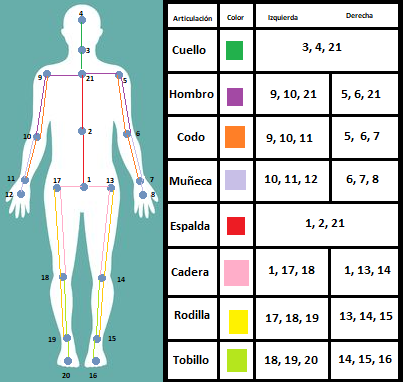
\includegraphics[width=280px,height=180px]{graphics/EskeletanAngles.png} \\
	\textbf{Fuente:}Elaboraci\'on propia 
\end{figure}
\begin{formula}[h]
	\centering
	\caption{Rotaci\'on a un punto de articulaci\'on}
	\label{frm:rotEq}
	\begin{equation}
\begin{matrix}
arco_{a} = [joint_{a},joint_{b},joint_{c}]\\ 
joint_{b}^{'} = [a,joint_{b}x-joint_{a}x, joint_{b}y-joint_{a}y]\\ 
joint_{c}^{'} = [a,joint_{c}x-joint_{a}x, joint_{c}y-joint_{a}y]
\end{matrix}
	\end{equation}
	\textbf{Fuente:} Traslaci\'on de ejes \cite[p.~982]{aguilar2009matematicas}
\end{formula}  
\begin{formula}[h]
	\centering
	\caption{flexibilidad de una articulaci\'on}
	\label{frm:angleArc}
	\begin{equation}
\begin{matrix}
joint_{b}^{'} \cdot joint_{c}^{'}=  joint_{b}^{'}x \, joint_{c}^{'}x + joint_{b}^{'}y \, joint_{c}^{'}y \\ 
\\ 
\left | joint \right |= \sqrt{ {joint_{x}}^{2} + {joint_{y}}^{2}}\\ 
\\ 
\alpha _{arco_{a}} = \frac{joint_{b}^{'} \cdot joint_{c}^{'}}{\left | joint_{b}^{'}\right |\left |  joint_{c}^{'}\right |}
\end{matrix}
	\end{equation}
	\textbf{Fuente:} \'Angulo entre dos vectores \cite[p.~591]{stewart2013precalculus}
\end{formula}  
\begin{table}[H]
\begin{center}
\caption{Definiciones de variables independientes del octavo objetivo}
\label{tab:defoi8}
\begin{tabular}{|l|l|l|}
\hline
Enumeraci\'on & Definici\'on Operacional & Definici\'on conceptual \\
\hline
\ref{vr:8oi:indep}.A & \begin{tabular}[c]{@{}l@{}}Variable que permite realizar \\ el movimiento en las articulaciones \\ del cuerpo humano  \end{tabular} &  \begin{tabular}[c]{@{}l@{}}De acuerdo a las variables \\ de un movimiento (ver secci\'on \ref{mt:mf:var})\\ la flexibilidad ayuda a la precisi\'on,\\ balance y coordinaci\'on \\ de un movimiento\end{tabular}\\
\hline
\end{tabular}
\end{center}
\textbf{Fuente:} Elaborado por el autor de tesis
\end{table}
\section{Alcances y limitaciones}
\begin{itemize}
\item Se trabajar\'a con los equipos deportivos que entrenan dentro de la Universidad Rafael Land\'ivar.
\item Se instalar\'a el prototipo de toma de datos del proyecto, en los lugares de entrenamiento de cada equipo deportivo.
\item En cada lugar de entrenamiento debe haber una fuente de energ\'ia para conectar la computadora port\'atil y el sensor Kinect.
\item Cada deporte de la Universidad Rafael Land\'ivar, trabajan  3 d\'ias de entrenamiento competitivo (combates, partidos, rutinas) y un d\'ia de entrenamiento de aprendizaje (e.g. t\'ecnicas, movimientos, dominio). Por lo tanto, se recolectar\'a los datos durante el entrenamiento de aprendizaje de cada deporte.
\item Se utilizar\'a un sensor Kinect, la cual se posicionar\'a de manera que genere completamente el seguimiento del esqueleto.
\item Por cada deporte seleccionado, se analizar\'a un movimiento que no salga del campo de visi\'on del sensor Kinect.
\item Antes de la captura de datos, el atleta debe realizar el calentamiento que realiza constantemente.
\item Durante todas las etapas, el atleta debe estar en un entorno adecuado y as\'i mismo con la vestimenta correcta (e.g. Ropa deportiva).
\item Debe estar presente el entrenador o profesional, durante la captura de datos.
\item  La captura de datos se realizar\'a de manera individual (Atleta por atleta).
\item  La recolecci\'on de datos se centra en el seguimiento del esqueleto del atleta.
\item La validaci\'on de datos se realizar\'a con los atletas que no participar\'an en la etapa de recolecci\'on de datos.
\item La actividad f\'isica se contabilizar\'a por medio de las repeticiones de un  movimiento, ejecutados durante una rutina tabata.
\item Las rutinas tabata ser\'an realizadas conjuntamente por el entrenador y el investigador.
\item Las aplicaciones que implemente el seguimiento del esqueleto ser\'an desarrolladas para el sistema operativo windows 10.
\item \'Unicamente se visualizar\'a los resultados de la rutina actual (no se llevar\'an los registros hist\'oricos de resultado de un atleta).
\end{itemize}
\section{Aportes}
El presente proyecto aporta un software que identifica si una persona esta en movimiento, con la ayuda de dos \'areas de estudios:
\begin{itemize}
	\item \textbf{\gls{visArt}:} La investigaci\'on brinda informaci\'on sobre el funcionamiento del sensor Kinect y sus respectivas herramientas, las cuales ayudan a crear una base de datos de reconocimiento de gesturas y posturas, usando la tecnolog\'ia de m\'aquinas de aprendizajes -i.e. Random Forest Regression-, con la finalidad de crear un modelo que detecta el movimiento de una persona.
	\item \textbf{Salud y deporte para el control del sedentarismo:} La investigaci\'on aporta tres movimientos que se puede ejecutar en rutinas de alta intensidad, que permite estimular el cuerpo humano para cumplir las recomendaciones de la organizaci\'on mundial de la salud.
\end{itemize}
